\chapter{Getting Started}

\section{Host System Requirements}

The majority of development is performed on Linux operating systems (primarily Debian) so this is the most well
tested platform, however Windows and Mac OS are also supported.

Any 64-bit Intel or AMD processor, or Apple Silicon Mac, should be able to run ngscopeclient. If AVX2 and/or AVX512F
support is present ngscopeclient will use special optimized versions of some signal processing functions, however
neither instruction set is required. Other (non Apple Silicon) ARM64 platforms may work if a compatible GPU is
available, but have not been tested. We don't actively test on 32-bit platforms due to the significant RAM
requirements, but we won't stop you from trying and would love to hear if you get it working.

A mouse with scroll wheel, or touchpad with scroll gesture support, is mandatory to enable full use of the UI. We may
explore alternative input methods for some UI elements in the future.

Any GPU with Vulkan support should be able to run ngscopeclient, however Vulkan 1.2 will deliver better performance.
The minimum supported GPUs are:
\begin{itemize}
\item NVIDIA: Maxwell architecture (GeForce GTX 700 series and newer, February 2014)
\item AMD: GCN based (Radeon HD 7000 and newer, January 2012)
\item Intel: Iris Plus 540 or HD Graphics 520 (Skylake, August 2015)
\item Apple: all Apple Silicon devices (M1 and newer). Newer Intel devices with Metal support should work but have not
been tested.
\end{itemize}

Note that many virtual machine graphics stacks (e.g. VMWare) do not provide Vulkan unless a PCIe passthrough GPU is
being used.

The minimum RAM requirement to launch ngscopeclient is relatively small; however, actual memory consumption is
heavily dependent on workload and can easily reach into the tens of gigabytes when doing complex analysis on many
channels with deep history.

Typical RAM consumption examples:
\begin{itemize}
\item Default configuration with demo scope (4 channels 100K points, 10 waveforms of history, no analysis): 250 MB
\item 4M point live streaming with 10 waveforms of history, eye pattern, 8B/10B decode, and jitter histogram: 650 MB
\item Single 512M point waveform, no analysis or history: 2.1 GB
\item 512M point P/N channel waveforms with CDR and eye pattern, no history: 8.3 GB
\end{itemize}

Large amounts of GPU RAM are required for working with deep waveforms, especially if you intend to perform
complex analysis on them. Analog waveforms are stored in 32-bit floating point format internally, so a single 256
megapoint waveform will consume 1GB of GPU memory. Intermediate results in multi-step filter pipelines require GPU
memory as well, even if not displayed.

The maximum supported waveform size depends on your Vulkan implementation but is typically $2^32$ bytes (4 GB). This
translates to one gigapoint analog or four gigapoints digital.

\section{Instrument Support}

ngscopeclient uses the libscopehal library to communicate with instruments, so any libscopehal-compatible hardware
should work with ngscopeclient. See the \hyperref[sec:scope-drivers]{Oscilloscope Drivers} section for more details on
which hardware is supported and how to configure specific drivers.

\section{Installation}

\subsection{Official Releases}

Prebuilt binary packages are available for some of our supported platforms.

The latest released binaries can be downloaded from GitHub at (FIXME url here).

\subsection{Development Builds}

If you are feeling adventurous and want to try bleeding-edge code, or are testing a fix at a developer's request,
packages for a limited set of platforms (currently Ubuntu 20.04, 22.04, 24.04, and Windows) are automatically built
each commit as part of the GitHub CI pipeline.

To access development packages, log into GitHub (sorry, development binaries are not available to
anonymous users - this is on GitHub's end and not under our control) and go to
\url{https://github.com/ngscopeclient/scopehal-apps/actions}. Select build-ubuntu or build-windows as appropriate,
click the commit you wish to test, and download the appropriate .msi or .deb package.

\section{Compilation}

ngscopeclient can be compiled on Linux, macOS, and Windows. While the compilation process is generally similar, various
steps differ among platform and distro.

\subsection{Linux}
\begin{enumerate}

\item Install dependencies.

\subsubsection{Debian}

Basic requirements:
\begin{lstlisting}[language=sh, numbers=none]
sudo apt-get install build-essential git cmake pkgconf libgtkmm-3.0-dev \
libcairomm-1.0-dev libsigc++-2.0-dev libyaml-cpp-dev catch2 libglfw3-dev curl xzip libhidapi-dev
\end{lstlisting}

On Debian bookworm and later, you can use system-provided Vulkan packages. Skip this on Debian bullseye, or if you
choose to use the Vulkan SDK instead:
\begin{lstlisting}[language=sh, numbers=none]
sudo apt-get install libvulkan-dev glslang-dev glslang-tools spirv-tools glslc
\end{lstlisting}

On Debian bullseye, you will need cmake from backports:
\begin{lstlisting}[language=sh, numbers=none]
sudo bash -c 'echo "deb http://deb.debian.org/debian bullseye-backports main" >> \
/etc/apt/sources.list.d/bullseye-backports.list'
sudo apt-get update
sudo apt-get install cmake/bullseye-backports
\end{lstlisting}

To build the LXI component (needed if you have LXI- or VXI-11-based instruments):
\begin{lstlisting}[language=sh, numbers=none]
sudo apt install liblxi-dev libtirpc-dev
\end{lstlisting}

For GPIB, you will need to install Linux-GPIB; instructions for this are out of scope here.

To build the documentation, you will also need LaTeX packages:
\begin{lstlisting}[language=sh, numbers=none]
sudo apt install texlive texlive-fonts-extra texlive-extra-utils
\end{lstlisting}

\subsubsection{Ubuntu}

Basic requirements:
\begin{lstlisting}[language=sh, numbers=none]
sudo apt install build-essential git cmake pkgconf libgtkmm-3.0-dev \
libcairomm-1.0-dev libsigc++-2.0-dev libyaml-cpp-dev catch2 libglfw3-dev curl xzip libhidapi-dev
\end{lstlisting}

On Ubuntu 22.10 and earlier (including 20.04 and 22.04), you will need to use the Vulkan SDK.
Instructions for installing this are in a later step. On Ubuntu 23.04 and later, you can instead
use system-provided Vulkan packages:
\begin{lstlisting}[language=sh, numbers=none]
sudo apt-get install libvulkan-dev glslang-dev glslang-tools spirv-tools glslc
\end{lstlisting}


To build the LXI component (needed if you have LXI- or VXI-11-based instruments):
\begin{lstlisting}[language=sh, numbers=none]
sudo apt install liblxi-dev libtirpc-dev
\end{lstlisting}

For GPIB, you will need to install Linux-GPIB; instructions for this are out of scope here.

To build the documentation, you will also need LaTeX packages:
\begin{lstlisting}[language=sh, numbers=none]
sudo apt install texlive texlive-fonts-extra texlive-extra-utils
\end{lstlisting}


\subsubsection{Fedora}
Basic requirements:
\begin{lstlisting}[language=sh, numbers=none]
sudo dnf install git gcc g++ cmake make pkgconf cairomm-devel gtk3-devel \
libsigc++30-devel yaml-cpp-devel catch-devel glfw-devel libhidapi-dev
\end{lstlisting}

System-provided Vulkan packages. Skip these if you choose to use the Vulkan SDK instead:
\begin{lstlisting}[language=sh, numbers=none]
sudo dnf install vulkan-headers vulkan-loader-devel glslang-devel  glslc \
libshaderc-devel spirv-tools-devel
\end{lstlisting}

To build the LXI component (needed if you have LXI- or VXI-11-based instruments):
\begin{lstlisting}[language=sh, numbers=none]
sudo dnf install liblxi-devel libtirpc-devel
\end{lstlisting}

For GPIB, you will need to install Linux-GPIB; instructions for this are out of scope here.

To build the documentation, you will also need LaTeX packages:
\begin{lstlisting}[language=sh, numbers=none]
sudo dnf install texlive
\end{lstlisting}

\subsubsection{Alpine Linux}

As Alpine Linux uses musl libc, you will need to use system-provided Vulkan packages, and not the Vulkan SDK.
\begin{lstlisting}[language=sh, numbers=none]
apk add git gcc g++ cmake make pkgconf cairomm-dev gtk+3.0-dev libsigc++-dev \
yaml-cpp-dev catch2-3 vulkan-loader-dev glslang-dev glslang-static glfw-dev \
shaderc-dev spirv-tools-dev libhidapi-dev
\end{lstlisting}

If you are using an older stable release (such as CentOS 7), you may need to install some dependencies from source.

\item Install Vulkan SDK:

In many cases, you can install the SDK components from distro-provided repositories, which is covered above. When
possible, this is preferred over installing the Vulkan SDK. If you choose not to, or are running a Linux distro that
does not provide these packages (for instance, Debian Bullseye, Ubuntu versions prior to 23.04, or other stable
distros), the following instructions cover installing and loading the Vulkan SDK.

The latest tested SDK at the time of documentation update is version 1.3.275.0. Newer SDKs are supported, but breaking
changes sometimes take place.
If you are using a newer SDK and run into problems, please file a bug report.

If you are using Ubuntu 20.04 or 22.04, you may install the
\href{https://packages.lunarg.com}{.deb packaged SDK release} instead of following the instructions below. This may
work for Debian as well but is not supported.

Alternatively, to use the tarball packaged SDK, download and unpack the tarball.
\href{https://vulkan.lunarg.com/sdk/home}{You can manually download the SDK}, or do the following:
\begin{lstlisting}[language=sh, numbers=none]
cd ~
mkdir VulkanSDK
cd VulkanSDK
curl -LO 'https://vulkan.lunarg.com/sdk/download/1.3.275.0/linux/vulkansdk-linux-x86_64-1.3.275.0.tar.xz'
tar xfv vulkansdk-linux-x86_64-1.3.275.0.tar.xz
\end{lstlisting}

And then source the `setup-env.sh` file:
\begin{lstlisting}[language=sh, numbers=none]
source "$HOME/VulkanSDK/1.3.275.0/setup-env.sh"
\end{lstlisting}

When using the tarball-packaged SDK, you will need to source the `setup-env.sh` file any time you want to compile
or run ngscopeclient. For convenience, you can add this to your `.bash\_profile` or equivalent:
\begin{lstlisting}[language=sh, numbers=none]
echo "source \"$HOME/VulkanSDK/1.3.275.0/setup-env.sh\"" >> ~/.bash_profile
\end{lstlisting}

\item Build scopehal and scopehal-apps:

\begin{lstlisting}[language=sh, numbers=none]
cd ~
git clone --recursive https://github.com/ngscopeclient/scopehal-apps.git
cd scopehal-apps
mkdir build
cd build
cmake .. -DCMAKE_BUILD_TYPE=Release
make -j4
\end{lstlisting}

\end{enumerate}

\subsection{macOS}
\begin{enumerate}

\item Install dependencies.

You will need Xcode (either from the App Store or the Apple developer site); after installing, run it once for it
to install system components. This provides gcc, g++, make, and similar required packages.

With Homebrew (\href{https://brew.sh}{brew.sh}):

\item Basic requirements:
\begin{lstlisting}[language=sh, numbers=none]
brew install pkg-config cairomm libsigc++ glfw cmake yaml-cpp glew catch2 libomp hidapi
\end{lstlisting}

\item Vulkan SDK components (skip if using the Vulkan SDK):
\begin{lstlisting}[language=sh, numbers=none]
brew install vulkan-headers vulkan-loader glslang shaderc spirv-tools molten-vk
\end{lstlisting}

\item Alternatively, install the Vulkan SDK:

 \href{https://vulkan.lunarg.com/sdk/home}{Download and install the Vulkan SDK.}.
The latest tested SDK at the time of documentation update is version 1.3.275.0. Newer SDKs are supported, but breaking
changes sometimes take place.
If you are using a newer SDK and run into problems, please file a bug report.

And then source the `setup-env.sh` file:
\begin{lstlisting}[language=sh, numbers=none]
source "$HOME/VulkanSDK/1.3.275.0/setup-env.sh"
\end{lstlisting}

When using the SDK, you will need to source the `setup-env.sh` file any time you want to compile or run ngscopeclient.
For convenience, you can add this to your `.zprofile` or equivalent:
\begin{lstlisting}[language=sh, numbers=none]
echo "source \"$HOME/VulkanSDK/1.3.275.0/setup-env.sh\"" >> ~/.zprofile
\end{lstlisting}

\item Build scopehal and scopehal-apps:

\begin{lstlisting}[language=sh, numbers=none]
cd ~
git clone --recursive https://github.com/ngscopeclient/scopehal-apps.git
cd scopehal-apps
mkdir build
cd build
cmake .. -DCMAKE_BUILD_TYPE=Release -DCMAKE_PREFIX_PATH="$(brew --prefix);$(brew --prefix)/opt/libomp"
make -j4
\end{lstlisting}

\end{enumerate}

\subsection{Windows}

On Windows, we make use of the MSYS2 development environment, which gives us access to the MingGW-w64 toolchain.
Since this toolchain allows ngscopeclient to be compiled as a native Windows application, the project might be run
outside of MSYS2.

\subsubsection{Building from source}

\begin{enumerate}

\item Download and install MSYS2. You can download it from \href{https://www.msys2.org/}{msys2.org} or
\href{https://github.com/msys2/msys2-installer/releases}{github.com/msys2/msys2-installer/releases}\\


The following steps can be done in any MSYS-provided shell.

% \item If you would like to build the installer package, install WIX Toolset from https://wixtoolset.org/docs/wix3/

\item Install git and the toolchain:
\begin{lstlisting}[language=sh, numbers=none]
pacman -S git wget mingw-w64-ucrt-x86\_64-cmake mingw-w64-ucrt-x86\_64-toolchain
\end{lstlisting}

\item Install general dependencies:
\begin{lstlisting}[language=sh, numbers=none]
pacman -S mingw-w64-ucrt-x86\_64-libsigc++ mingw-w64-ucrt-x86\_64-cairomm mingw-w64-ucrt-x86\_64-yaml-cpp mingw-w64-ucrt-x86\_64-glfw mingw-w64-ucrt-x86\_64-catch mingw-w64-ucrt-x86\_64-hidapi
\end{lstlisting}

\item Install Vulkan dependencies:
\begin{lstlisting}[language=sh, numbers=none]
pacman -S mingw-w64-ucrt-x86\_64-vulkan-headers mingw-w64-ucrt-x86\_64-vulkan-loader mingw-w64-ucrt-x86\_64-shaderc \
mingw-w64-ucrt-x86\_64-glslang mingw-w64-ucrt-x86\_64-spirv-tools
\end{lstlisting}

\item Install FFTS:
\begin{lstlisting}[language=sh, numbers=none]
pacman -S mingw-w64-ucrt-x86\_64-ffts
\end{lstlisting}


\item Check out the code

\begin{lstlisting}[language=sh, numbers=none]
cd ~
git clone --recursive https://github.com/ngscopeclient/scopehal-apps
\end{lstlisting}

All following steps are to be done in a UCRT64 shell.

\item Build manually:
\begin{lstlisting}[language=sh, numbers=none]
cd scopehal-apps
mkdir build
cd build
cmake ..
ninja -j4
\end{lstlisting}

\item Optional, to build MSI installer:

Download and install WiX Toolset.\\
You can download it from \href{https://github.com/wixtoolset/wix3/releases}{https://github.com/wixtoolset/wix3/releases}\\
If you install it to the path \texttt{"C:\textbackslash Program Files (x86)\textbackslash WiX Toolset v3.14"} run the following cmake command instead of \texttt{cmake ..} mentioned earlier:

\begin{lstlisting}[language=sh, numbers=none]
cmake .. -DWIXPATH="C:\Program Files (x86)\WiX Toolset v3.14\bin"
\end{lstlisting}

\texttt{ninja} compilation will now generate the installer after binaries.

% \item Alternatively, Execute makepkg-mingw in subdir MSYS2:

% \begin{lstlisting}[language=sh, numbers=none]
% cd ~/scopehal-apps/msys2

% MINGW\_ARCH=mingw64 makepkg-mingw --noconfirm --noprogressbar -sCLf
% \end{lstlisting}

% !and remove the -DBUILD\_TESTING=OFF flag from the PKGBUILD recipe in subdir
% msys2.

% \item Installing, copying binaries and running ngscopeclient.

% Since ngscopeclient is built using the MinGW toolchain, it depends on a rather large number of dynamic libraries.
% The recommended procedure is to install the package generated by makepkg-mingw on a MinGW64 shell:

% MSVC build

% Install vcpkg
% Integrate vcpkg - vcpkg integrate install

% run cmake (replace VCPKG_ROOT with the install path of vcpkg):
% cmake -B build -S . -DCMAKE_TOOLCHAIN_FILE=VCPKG_ROOT\scripts\buildsystems\vcpkg.cmake

% Open Visual Studio and build the software.

% \begin{lstlisting}[language=sh, numbers=none]
% cd ~
% cd msys2
% pacman -U *.zst
% \end{lstlisting}

% This is equivalent to the package installed through \lstinline{pacman -S}, but it's built from the checked out commit,
% instead of the pinned version available from MSYS2 repositories.

% The \lstinline{*.zst} package includes metadata about the dependencies.
% Therefore, when installed through \lstinline{pacman}, those will be installed automatically.
% However, some users might want to use ngscopeclient outside of MSYS2.
% In those cases, it needs to be installed first, and then a tarball/zipfile can be created by collecting all the dependencies.
% This last approach is not officially supported yet.

\item Run scopehal and scopehal-apps:

Building scopehal and scopehal-apps with MSYS2 will install requierd dependencies in MSYS2's libpath, that's why ngscopeclient has to be launched from a MSYS2 shell (use MSI installer to generate a standalone package).

The binaries can be found in the build directory, such as ngscopeclient in \$HOME/scopehal-apps/build/src/ngscopeclient.

Use the following commands to run ngscopeclient:
\begin{lstlisting}[language=sh, numbers=none]
cd src/ngscopeclient/
./ngscopeclient.exe
\end{lstlisting}

Or with some debug options:
\begin{lstlisting}[language=sh, numbers=none]
./ngscopeclient.exe --debug --trace SCPISocketTransport
\end{lstlisting}



\end{enumerate}

\section{Running ngscopeclient}

When running ngscopeclient with no arguments, an empty session (Fig. \ref{empty-window}) is created. To perform useful
work, you can:
\begin{itemize}
\item Open a saved session and reconnect to the instruments (\menustyle{File | Open Online})
\item Open a saved session without reconnecting to the instruments (\menustyle{File | Open Offline})
\item Open a recently used session (\menustyle{File | Recent Files})
\item Import waveforms from a third party file format(\menustyle{Add | Import})
\item Connect to an instrument (\menustyle{Add | Oscilloscope}, \menustyle{Add | Multimeter}, etc.)
\item Generate a synthetic waveform (\menustyle{Add | Generate})
\end{itemize}

\begin{figure}[h]
\centering
	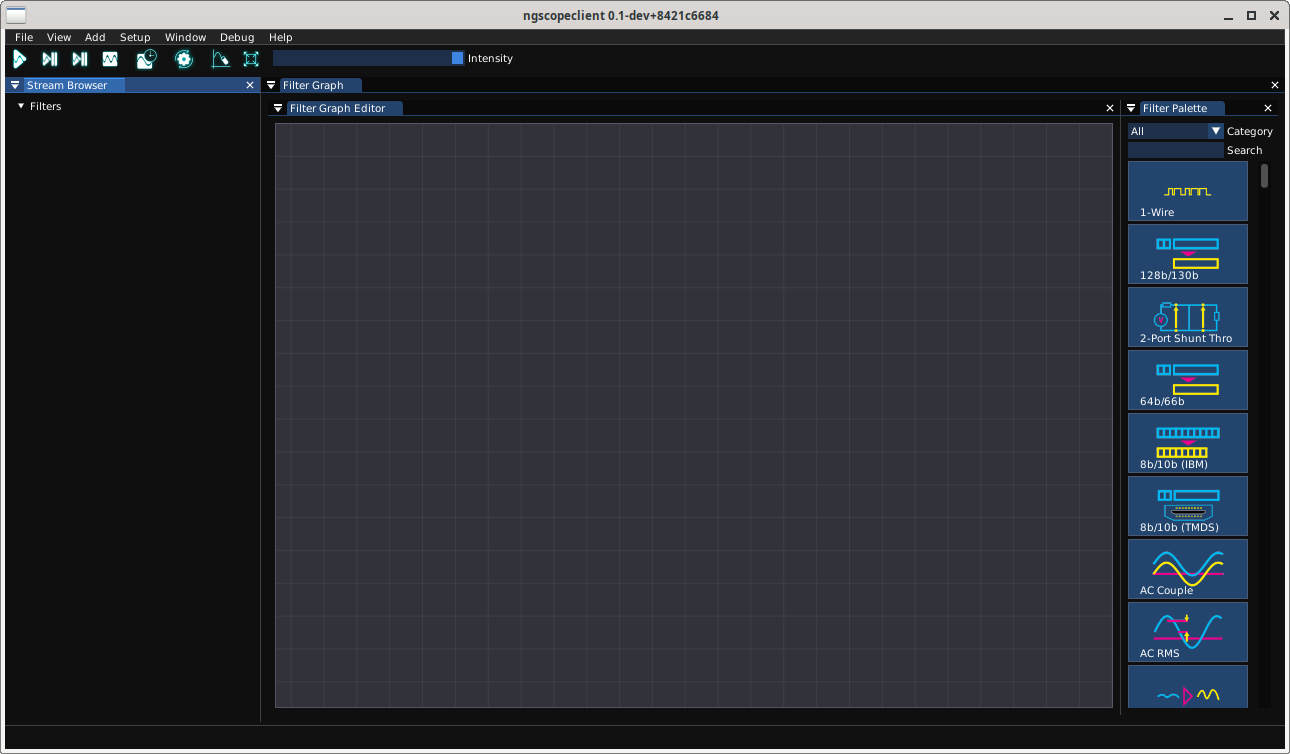
\includegraphics[width=12cm]{ng-images/empty-window.png}
\caption{Empty ngscopeclient session}
\label{empty-window}
\end{figure}

% TODO: add this section once these are implemented
\begin{comment}

\subsection{Configuration arguments}

Most of these arguments are intended for developers, but they can help troubleshoot unusual bugs.

\begin{itemize}

\item \texttt{-{}-noavx2}\\
Do not use AVX2 vector optimizations even if the CPU supports it.

\item \texttt{-{}-noavx512f}\\
Do not use AVX512F vector optimizations even if the CPU supports it.

\item \texttt{-{}-noglint64}\\
Do not use \texttt{GL\_ARB\_gpu\_shader\_int64} even if the GPU supports it.

\item \texttt{-{}-nogpufilter}\\
Do not use Vulkan (GPU accelerated) implementations of filter blocks, revert to software fallback.

\end{itemize}

\end{comment}

\subsection{Console verbosity arguments}

ngscopeclient takes standard liblogtools arguments for controlling console debug verbosity.

If no verbosity level is specified, the default is ``notice" (3). (We suggest using \texttt{-{}-debug} for routine use
until the v1.0 release to aid in troubleshooting.)

\begin{itemize}

\item \texttt{-{}-debug}\\
Sets the verbosity level to ``debug" (5).

\item \texttt{-l [file]}, \texttt{-{}-logfile [file]}\\
Writes a copy of all log messages to \texttt{file}. This is preferred over simply redirecting output with pipes, as
console escape sequences are stripped from the file log output.

\item \texttt{-L [file]}, \texttt{-{}-logfile-lines [file]}\\
Same as \texttt{-{}-logfile} except line buffering is turned on.

\item \texttt{-q}, \texttt{-{}-quiet}\\
Reduces the verbosity level by one. Can be specified more than once to lower verbosity by several steps.

\item \texttt{-{}-trace [class]}, \texttt{-{}-trace [class::function]} \\
Enables extra debug output from the class \texttt{class} or the function \texttt{class::function}. Has no effect unless
\texttt{-{}-debug} is also specified.

\item \texttt{-{}-stdout-only}\\
Sends all logging output to stdout. By default, error (level 1) and warning (level 2) messages go to stderr.

\item \texttt{-{}-verbose}\\
Sets the verbosity level to ``verbose" (4).

\end{itemize}

% TODO: add this section once these are implemented
\begin{comment}
\subsection{File arguments}
\label{import}

The file extension is used to determine the format. File extensions are case sensitive and must be lowercase to be
correctly interpreted.

\begin{itemize}
\item \texttt{[file.scopesession]}
Loads a saved session.

\item \texttt{[file.bin]} \\
Imports waveform data from the binary format used by Agilent, Keysight, and Rigol oscilloscopes.

\item \texttt{[file.complex]} \\
Imports complex I/Q data from a file. The file must contain interleaved (I, Q) pairs in either 8-bit signed/unsigned
integer, 16-bit signed integer, 32-bit normalized floating point, or 64-bit normalized floating point format.

The default format is 8 bit signed integer and may be changed from the filter graph editor or channel properties dialog
once the file is loaded. There is currently no way to specify other formats on the command line.

\item \texttt{[file.csv]} \\
Imports sample data from a CSV (comma-separated-value) file. More than one CSV file can be loaded at once (displayed as
separate points in history) by specifying multiple file names as long as they have identical column schemas.

Lines starting with a '\#' character are treated as comments and generally ignored by the parser. (If the comment format
matches that used by Digilent's WaveForms utility, timestamps and other metadata are extracted from the comments.)

If the first row of the CSV contains non-numeric characters, it is treated as a header row. Header content in the
timestamp column is ignored; headers in other columns are used as channel names in the imported waveform.

The first column of the CSV must contain sample timestamps, in seconds. Scientific notation is supported. Timestamps
must be monotonic (each row must have a timestamp strictly greater than that of the previous row).

ngscopeclient uses a heuristic to detect uniformly sampled waveforms, which enabled certain optimizations for display
and signal processing. If the standard deviation of intervals between samples is less than 1\% of the average sample
interval, the waveform is assumed to be uniformly sampled and timestamps are rounded to the nearest multiple of the
average interval. If the deviation is greater, the waveform is assumed to be sparsely sampled and timestamps are not
modified.

\item \texttt{[file.trc]} \\
Imports waveform data from a Teledyne LeCroy .trc binary waveform file.

\item \texttt{[file.vcd]} \\
Imports digital waveform data from a VCD (value change dump) file, typically created by a logic analyzer or HDL
simulator.

\item \texttt{[file.wav]} \\
Imports sample data from a WAV file.

\item \texttt{[file.wfm]} \\
Imports sample data from a Tektronix .wfm file. This import filter is still experimental and may not support all
features of the .wfm file format yet. If you have trouble importing some .wfm files please file a ticket on GitHub.

%%%%%%%%%%%%%%%%%%%%%%%%%%%%%%%%%%%%%%%%

\item \texttt{-{}-nodata}\\
When loading a .scopesession file, load settings only and not saved waveform data.

\item \texttt{-{}-reconnect}\\
When loading a .scopesession file, reconnect to the instrument and resume remote control. Current instrument settings
are overwritten with the configuration from the saved session.

\item \texttt{-{}-retrigger}\\
When loading a .scopesession file, arm the trigger immediately. has no effect unless \texttt{-{}-reconnect} is also
specified.

\end{itemize}

\subsection{Instrument arguments}

Example:
\begin{lstlisting}[language=sh, numbers=none]
./ngscopeclient --debug \
	mylecroy:lecroy:vicp:myscope.example.com:1234 \
	myrigol:rigol:lan:rigol.example.com
\end{lstlisting}

\begin{itemize}
\item \texttt{[connection string]} \\
Connects to the specified instrument. By default, all channels are enabled and displayed.

\end{itemize}

Each instrument is described by a ``connection string" containing four colon-separated fields.

\begin{itemize}
\item Nickname. This can be any text string not containing spaces or colons. If you have only one instrument it's
largely ignored, but when multiple instruments are present channel names in the UI are prefixed with the nickname to
avoid ambiguity.
\item Driver name. This is a string identifying the command protocol the scope uses. Note that not all
scopes from the same vendor will use the same command set or driver!
\item Transport. This is is a string describing how the driver connects to the scope (e.g. RS232 or Ethernet)
\item Arguments for the driver identifying the device to connect to, separated by colons. This varies by driver but is
typically a hostname:port combination, TTY device path, or similar.
\end{itemize}

\end{comment}
